\documentclass{ieeeojies}
\usepackage{cite}
\usepackage{amsmath,amssymb,amsfonts}
\usepackage{algorithmic}
\usepackage{graphicx}
\usepackage{textcomp}
\usepackage{array}
\usepackage[table]{xcolor}
\usepackage{multirow}
\usepackage{multicol}
\usepackage{float}

\def\BibTeX{{\rm B\kern-.05em{\sc i\kern-.025em b}\kern-.08em
    T\kern-.1667em\lower.7ex\hbox{E}\kern-.125emX}}

\begin{document}
\title{FORECASTING THE CURRENCY PRICE USING STATISTICAL MODELS AND MACHINE LEARNING}

\author{\uppercase{Trinh Thi My Chung}\authorrefmark{1},
\uppercase{Tran Phuong Anh\authorrefmark{2}, and Che Duy Khang 3}\authorrefmark{3}}

\address[1]{Faculty of Information Systems, University of Information Technology, (e-mail: 21520653@gm.uit.edu.vn)}
\address[2]{Faculty of Information Systems, University of Information Technology, (e-mail: 21520595@gm.uit.edu.vn)}
\address[3]{Faculty of Information Systems, University of Information Technology, (e-mail: 21522187@gm.uit.edu.vn)}

\markboth
{Team 4 \headeretal: Trinh Thi My Chung, Tran Phuong Anh, Che Duy Khang}
{Team 4 \headeretal: Trinh Thi My Chung, Tran Phuong Anh, Che Duy Khang}

\begin{abstract}

The currency market plays a crucial role in global finance, facilitating transactions between different countries and enabling international trade. Accurate forecasting of currency prices is essential for businesses and investors to make informed decisions. This study focuses on forecasting the future prices of major currencies using statistical models and machine learning algorithms. By analyzing historical data and leveraging advanced techniques, we aim to develop reliable prediction models for currency prices. Additionally, the integration of machine learning methods enhances the accuracy and efficiency of the forecasting process. This research contributes to the field by providing insights into the application of statistical models and machine learning in currency price forecasting, ultimately aiding businesses and investors in managing currency-related risks and optimizing their financial strategies.
\end{abstract}

\begin{keywords}
\end{keywords}

\titlepgskip=-15pt

\maketitle

\section{Introduction}
\label{sec:introduction}
The currency price, often referred to as the exchange rate between different national currencies, plays a crucial role in global financial markets and economies. Its fluctuations have significant impacts on various aspects of the economy, including trade, investment, and banking. While currency price movements can present opportunities for investors and businesses, they also introduce uncertainties and risks.\par
\noindent
Traditionally, forecasting currency prices has been challenging due to the complex and unpredictable nature of the forex market. However, the advent of machine learning has opened new possibilities in this field. Machine learning algorithms excel at processing large volumes of data and identifying complex patterns that may not be discernible to humans.\par
\noindent
In recent years, several algorithms have gained prominence in currency price forecasting. Exponential Smoothing State Space Model (ETS), Stacking Model, and PatchTST are among the notable ones. ETS provides a framework for modeling and forecasting time series data, while Stacking Model combines multiple models to improve predictive accuracy. PatchTST, on the other hand, utilizes a patch-based approach for time series forecasting, leveraging both local and global patterns in the data.\par
\noindent
By leveraging statistical models and machine learning techniques for currency price forecasting, significant benefits can be derived for investors, businesses, and even entire nations. Understanding market trends and fluctuations enables informed decision-making regarding investment, risk management, and business planning based on more accurate currency price forecasts.\\
\noindent
This article explores the application of statistical models and machine learning algorithms in forecasting currency prices, highlighting their potential to enhance decision-making processes and drive economic growth.

\bigskip
\raggedright\textbf{GBP (Great British Pound)}
\bigskip


The British Pound Sterling (GBP), dating back to its introduction in the late 17th century, boasts a rich and enduring history. Its evolution from the establishment of paper money by the Bank of England to becoming one of the oldest and most widely traded currencies globally signifies its importance. Despite facing numerous economic and geopolitical challenges over the centuries, including wars and financial crises, the GBP has maintained its position as a symbol of stability and strength in the international financial system. Today, the GBP remains a cornerstone of global finance, with its exchange rate closely monitored by investors, traders, and policymakers worldwide. Its value reflects not only the economic health of the United Kingdom but also broader trends in international trade and finance. Thus, the GBP's legacy and resilience underscore its significance in shaping the landscape of global economics for generations.
\begin{figure}[h]
    \centering
    \includegraphics[scale=0.34]{GBP.png}
    \label{fig:us_image}
    \caption{Exchange rate of GBP from 2019 to 2024}
\end{figure}

\raggedright
\bigskip
\textbf{EUR (Euro)}
\bigskip

The Euro is the common currency of the member countries in the Eurozone, a monetary union consisting of 19 of the 27 European Union (EU) member states. It is widely used in trade and finance, serving as a primary medium of exchange for transactions within the Eurozone and beyond. The Euro's exchange rate is closely monitored by economists, investors, and policymakers, as it serves as a key indicator of the region's economic health and stability. Its value against other major currencies, such as the US dollar and the British pound, is often used as a benchmark for global trade and investment. Despite occasional fluctuations, the Euro has maintained a relatively stable exchange rate, contributing to its reputation for stability and credibility in the international financial system. This stability has attracted trust from investors and businesses worldwide, making the Euro one of the most widely accepted and respected currencies in the world.
\begin{figure}[h]
    \centering
    \includegraphics[scale=0.35]{Euro.png}
    \caption{Exchange rate of EUR from 2019 to 2024}
    \label{fig:euro_image}
\end{figure}


\bigskip
\textbf{EUR (Japanese Yen)}
\bigskip

The yen is the official currency of Japan and is widely recognized as one of the major currencies in the world. Its exchange rate is closely monitored in global financial markets due to Japan's significant role in international trade and finance. The yen's value can be influenced by various factors, including Japan's economic performance, monetary policies, and geopolitical developments.
\begin{figure}[h]
    \centering
    \includegraphics[scale=0.35]{YEN1.png}
    \label{fig:yen_image}
    \caption{Exchange rate of EUR from 2019 to 2024}
\end{figure}

\section{Related Works}
Accurately forecasting currency exchange rates has been an enormous challenge because of the complexity and dynamism of financial markets. Researchers have worked in this area so as to explore different methodologies to achieve reliable predictions. There have been many research articles on predicting currency exchange rate, such as:

Pengfei Liu et al. [1] study on currency exchange rate prediction by implementing multiple forecasting model to forecast and analyze the daily currency exchange rate of USD/RMB. This study uses CNN, STLSTM, AM model to estimate the accuracy of models. The experiments show that all three models above have higher forecasting accuracy and fitting degree that other models and they are appropriate for forecasting the closing price of the USD/RMB exchange rate.

M.S. Islam, E. Hossain [2] focus on forecasting the currency exchange rate by presenting a new model that combines two powerful neural networks used for time series prediction: Gated Recurrent Unit (GRU) and Long Short-Term Memory (LSTM). It is used for predicting future closing prices of FOREX currencies. The performance of the model is validated using MSE, RMSE, MAE and R2 score. Researchers applied the model to predict the closing price of four currency pairs in 10 and 30 minutes before the actual time. The model is considered a promising area and has a good predictive capability

Siyuan Liu et al. [3] research on predicting the USD/CNY exchange rate using the novel LASSO-BiLSTM-based ensemble learning method by integrating least absolute shrinkage and selection operator (LASSO) and bidirectional long short-term memory (LSTM). The model performed well and the LASSO-BiLSTM-based ensemble learning method demonstrated high potential in forecasting exchange rates

Qimian Zhu [4] has paper aims to forecast the change of exchange rate of USD/EUR in 2022 using ARIMA model. Researchers discussed the performance of the univariate ARIMA model and the multivariate regression model with ARIMA errors, i.e. four macroeconomic variables, influence the exchange rate incorporated in the AR part of the ARIMA model. The performance of model depends on the quality of the predicted predictors, which are the four macroeconomic variables in the study

Kamruzzaman et al. [5] apply ANNs to predict currency exchange rate of Australian Dollar against other currencies, such as US Dollar (USD), Great British Pound (GBP), Japanese Yen (JPY), Singapore Dollar (SGD), New Zealand Dollar (NZD) and Swiss Franc (CHF). The research focuses on three different ANNs based model, which is Standard Backpropagation (SBP), Scaled Conjugate Gradient (SCG) and Bayesian regularization (BPR). Five different indicators, which are Normalized Mean Square Error (NMSE), Mean Absolute Error (MAE), Directional Symmetry (DS), Correct Up
trend (CU) and Correct Down trend (CD), were used to compare the result of three models, for 35 and 65 weeks. The results show that SCG and BPR forecast more accurately than SBP and follow closely to the actual exchange rate, in term of the metrics calculated.


\section{Materials}
\subsection{Dataset}

This study will utilize historical exchange rate data of Euro (EUR) to Vietnamese Dong (VND), British Pound (GBP) to Vietnamese Dong (VND), and Japanese Yen (JPY) to Vietnamese Dong (VND) from 1/3/2019 to 1/3/2024. The dataset includes columns such as Date, Purchase Price, Sale Price, and Transfer Price. Since the objective is to forecast foreign currencies' sale prices, only data related to the Sale (VND) columns will be processed.

\subsection{Descriptive Statistics}
\begin{table}[H]
  \centering
  \caption{EUR-VND, GBP-VND, JPY-VND dataset’s Descriptive Statistics}
\begin{tabular}{|>{\columncolor{red!20}}c|c|c|c|}
    \hline
     \rowcolor{red!20} & EUR-VND & GBP-VND & JPY-VND \\ \hline
     Count & 1825 & 1825 & 1825 \\ \hline
     Mean & 26715.9 & 30411.2 & 200.8\\ \hline
     Std & 1062.08 & 1268.95 & 20.34\\ \hline
     Min & 23533 & 25979 & 166.27\\ \hline
     25\% & 26151 & 29537 & 179.55\\ \hline
     50\% & 26647 & 30448 & 210.46\\ \hline
     75\% & 27469 & 31311 & 217.99\\ \hline
     Max & 29180 & 33305 & 228.6\\ \hline
\end{tabular}
\end{table}

\begin{figure}[H]
    \centering
    \begin{minipage}{0.23\textwidth}
    \centering
    \includegraphics[width=1\textwidth]{bibliography/Figure/EUR_Boxplot.png}
    \caption{EUR-VND price's boxplot}
    \label{fig:1}
    \end{minipage}
    \hfill
    \begin{minipage}{0.23\textwidth}
    \centering
    \includegraphics[width=1\textwidth]{bibliography/Figure/EURhist.png}
    \caption{EUR-VND price's histogram}
    \label{fig:2}
    \end{minipage}
\end{figure}
From the descriptive statistics of the EUR-VND dataset, we can observe that the selling price of the Euro (EUR) to Vietnamese Dong (VND) currency pair from March 1, 2019, to March 1, 2024, exhibits a skewed distribution with the primary concentration around the mean and median values, but with uneven fluctuations.
\begin{figure}[H]
    \centering
    \begin{minipage}{0.23\textwidth}
    \centering
    \includegraphics[width=1\textwidth]{bibliography/Figure/GBPbox.png}
    \caption{GBP-VND price's boxplot}
    \label{fig:1}
    \end{minipage}
    \hfill
    \begin{minipage}{0.23\textwidth}
    \centering
    \includegraphics[width=1\textwidth]{bibliography/Figure/GBPhist.png}
    \caption{GBP-VND price's histogram}
    \label{fig:2}
    \end{minipage}
\end{figure}
From the descriptive statistics of the GBP-VND dataset, we can observe a certain level of volatility in the selling prices of the British Pound (GBP) to Vietnamese Dong (VND) currency pair from March 1, 2019, to March 1, 2024. Most selling prices are concentrated at lower levels, with some higher values contributing to an increase in standard deviation and causing a skewed right distribution on the histogram. 
\begin{figure}[H]
    \centering
    \begin{minipage}{0.23\textwidth}
    \centering
    \includegraphics[width=1\textwidth]{bibliography/Figure/JPYbox.png}
    \caption{JPY-VND price's boxplot}
    \label{fig:1}
    \end{minipage}
    \hfill
    \begin{minipage}{0.23\textwidth}
    \centering
    \includegraphics[width=1\textwidth]{bibliography/Figure/JPYhist.png}
    \caption{JPY-VND price's histogram}
    \label{fig:2}
    \end{minipage}
\end{figure}
From the descriptive statistics of the JPY-VND dataset, we can observe that the market selling price of the Japanese Yen (JPY) to Vietnamese Dong (VND) from March 1, 2019, to March 1, 2024, exhibits variability and fluctuations. The histogram of the data indicates instability and variability in the values. The boxplot of the dataset reveals that the majority of values concentrate at higher price levels.
\section{Methodology}

\subsection{Linear Regression}
Regression analysis is a tool for building mathematical and statistical models that characterize relationships between a dependent variable and one or more independent, or explanatory, variables, all of which are numerical. This statistical technique is used to find an equation that best predicts the y variable as a linear function of the x variables.
A multiple linear regression model has the form: 
\[Y=\beta_0+\beta_1X_1+\beta_2X_2+\cdots+\beta_kX_k+\varepsilon\]
Where:\\
	\indent\textbullet\ Y is the dependent variable (Target Variable).\\
	\indent\textbullet\ \(X_1, X_2, \ldots, X_k\) are the independent (explanatory) variables.\\
	\indent\textbullet\ \(\beta_0\) is the intercept term.\\
	\indent\textbullet\ \(\beta_1,..., \beta_k\) are the regression coefficients for the independent variables.\\
	\indent\textbullet\ \(\varepsilon\) is the error term.

 \subsection{AutoRegressive Integrated Moving Average (ARIMA)}
 ARIMA (AutoRegressive Integrated Moving Average) model is a form of regression analysis that gauges the strength of one dependent variable relative to other changing variables. The ARIMA model is used to make predictions about future values of the time series based on its past values. The ARIMA model consists of three parts including Autoregressive (AR), Integrated (I), and Moving Average (MA).\\ 
 
 The AR component with order p utilizes the preceding p values of the time series for current value prediction. The AR(p) model has the form:
 \[Y(t)=\alpha_0+\alpha_1Y(t-1)+\alpha_2Y(t-2)+\cdots+\alpha_pY(t-p)+\epsilon(t)\]
         Where:\\
	     \indent\textbullet\ Y(t) is current observed value.\\
          \indent\textbullet\ \(Y(t-1), Y(t-2), \ldots, Y(t-p)\) are past observed values.\\
          \indent\textbullet\ \(\alpha_0, \alpha_1, \ldots, \alpha_p\) are regression analysis parameters.\\
          \indent\textbullet\ \(\epsilon(t)\) is random forecasting error of the current period. The expected mean value is 0.\\
            
 Integrated (I) represents the differencing of raw observations to allow the time series to become stationary.\\
    \indent\textbullet\ First Difference I(1): dY(t) = Y(t) - Y(t-1)\\
    \indent\textbullet\ Second Difference I(2): dY(t) = Y(t) - 2Y(t-2) + Y(t-3)\\
 
The MA model with order q analyzes the past q forecast errors to anticipate the current value. The MA(q) model has the form:
  \[Y(t)=\beta_0+\epsilon(t)+\beta_1\epsilon(t-1)+\beta_2\epsilon(t-2)+\cdots+\beta_q\epsilon(t-q)\]
        Where:\\
	    \indent\textbullet\ Y(t) is current observed value.\\
            \indent\textbullet\ \(\epsilon(t)\) is random forecasting error of the current period. The expected mean value is 0.\\
            \indent\textbullet\ \(\epsilon(t-1), \epsilon(t-2), \ldots, \epsilon(t-q)\) are forecast error.\\
            \indent\textbullet\ \(\beta_0, \beta_1, \ldots, \beta_q\) mean values of Y(t) and moving average coefficients.\\
\subsection{Exponential Smoothing (ETS)}
Exponential smoothing is one of the most popular models used for demand forecasting in practice. It includes Error, Trend and Seasonal components, thus being called ‘ETS’ [6] 
There are three main methods to estimate exponential smoothing. They are: \\
    \indent\textbullet\ Simple exponential smoothing: used when the data has no trend and no seasonal pattern. \\
    \indent\textbullet\ Double exponential smoothing: used for forecasting the time series when the data has a linear trend and no seasonal pattern. \\
    \indent\textbullet\ Triple exponential smoothing: used for forecasting the time series when the data has both linear trend and seasonal pattern. This method is also called Holt-Winters exponential smoothing [7]
        \begin{align*}
        y_t &= l_{t-1} + b_{t-1} + s_{t-m} + \varepsilon_t \\
        l_t &= l_{t-1} + \alpha \varepsilon_t \\
        b_t &= b_{t-1} + \beta \varepsilon_t \\
        s_t &= s_{t-m} + \gamma \varepsilon_t
        \end{align*}
    \begin{description}
  \item[$y_t$] Actual value at time $t$.
  \item[$l_{t-1}$] Level estimate at time $t-1$.
  \item[$b_{t-1}$] Trend estimate at time $t-1$.
  \item[$s_{t-m}$] Seasonal component at time $t-m$ (where $m$ is the number of seasons).
  \item[$\varepsilon_t$] Random error at time $t$ [8]
\end{description}
\subsection{STACKING MODEL} 
Stacking Model, also known as Ensemble Learning, is a machine learning technique that combines multiple machine learning models to create a more accurate predictive model. \\
    \indent\textbullet\ Improved accuracy: Stacking Model can help improve the accuracy of predictions by combining the strengths of multiple different machine learning models. \\
    \indent\textbullet\ Reduced overfitting: Stacking Model can help reduce overfitting by using multiple different machine learning models to learn from the data. \\
    \indent\textbullet\ Increased flexibility: Stacking Model can be used with many different types of machine learning models, making it a versatile tool for different prediction tasks.

How Stacking Model Works:
\\
   \indent\textbullet\ Train base models: First, you need to train several base machine learning models on the data. These models can be of any type, such as linear regression, decision trees, random forests, etc. \\
   \indent\textbullet\ Create meta data: After training the base models, you need to create meta data. Meta data is a new dataset that includes the predictions of the base models as input data. \\
   \indent\textbullet\ Train meta model: Finally, you need to train a meta model on the meta data. The meta model will learn how to combine the predictions of the base models to.\\
Stacking Model is a powerful machine learning technique that can significantly improve the accuracy of predictive models. By combining the strengths of multiple different machine learning models, Stacking Model offers a flexible and effective approach to solving complex prediction tasks.

\subsection{Gated Recurrent Unit (GRU)} 
Gated Recurrent Unit (GRU) is a special kind of RNN (Recurrent Neural Network). For every element of a sequence, GRU performs a similar task. That is the reason for which it is called recurrent. [8]

A GRU cell consists of two gates: the update gate and the reset gate. These gates control how information flows through the cell, deciding what to keep and what to discard. The update gate determines how much of the past information needs to be passed along to the future. The reset gate determines how much of the past information to forget. These operations are performed by the following equations:
\begin{align*}
z_t &= \sigma\left( W^{(z)} x_t + U^{(z)} h_{t-1} \right) \\
r_t &= \sigma\left( W^{(r)} x_t + U^{(r)} h_{t-1} \right)
\end{align*}
\(h_t\) and \(h_{t-1}\) represent the output of the current and previous states, respectively, while \(r_t\) and \(z_t\) indicate the reset and update gates, respectively. \(\sigma\) is the logistic sigmoid function while \(W_r\) and \(U_r\) are the weight matrices.


\subsection{LSTM} 
XGBoost is an optimized distributed gradient boosting library designed for efficient and scalable training of machine learning models. It is an ensemble learning method that combines the predictions of multiple weak models to produce a stronger prediction. XGBoost stands for “Extreme Gradient Boosting” and it has become one of the most popular and widely used machine learning algorithms due to its ability to handle large datasets and its ability to achieve state-of-the-art performance in many machine learning tasks such as classification and regression.\\

 \item \textbf{Loss Function}:
        \[ \text{Loss} = \sum_{i=1}^{n} L(y_i, \hat{y}_i) + \sum_{k=1}^{K} \Omega(f_k) \]
        Where:
        \begin{itemize}
            \item $L(y_i, \hat{y}_i)$ is the loss function measuring the error between the predicted value $\hat{y}_i$ and the actual value $y_i$.
            \item $\Omega(f_k)$ is the penalty function measuring the complexity of the model, helping to prevent overfitting.
        \end{itemize}
        
    \item \textbf{Decision Trees}:
        Decision trees used in XGBoost are weak learners trained to minimize the loss function by optimizing values at nodes and splitting thresholds.
        
    \item \textbf{Regularization Terms}:
        $\Omega(f_k)$ typically includes two components: regularization terms to control the depth of trees ($T$) and reduce the number of leaf nodes ($J$):
        \[ \Omega(f_k) = \gamma T + \frac{1}{2} \lambda \sum_{j=1}^{J} w_j^2 \]
        Where:
        \begin{itemize}
            \item $\gamma$ and $\lambda$ are regularization parameters.
            \item $T$ is the depth of the tree.
            \item $w_j$ is the weight value of the $j$-th node.
        \end{itemize}
        
    \item \textbf{Optimization Objective}:
        The optimization objective of XGBoost is to minimize the loss function by finding the best trees $f_k$:
        \[ \text{Obj} = \sum_{i=1}^{n} L(y_i, \hat{y}_i) + \sum_{k=1}^{K} \Omega(f_k) \]

\subsection{Recurrent Neural Network (RNN)}
Recurrent Neural Network (RNN) is a type of neural network model designed to handle sequential data. The distinctive feature of RNNs is their ability to maintain information across time steps, allowing them to utilize information from previous steps to influence the processing of the current step. This makes RNNs particularly useful in applications where the order of data is important, such as natural language processing (NLP), machine translation, and time series forecasting. \\
RNNs operate by processing sequential data and maintaining a hidden state to capture information from previous time steps. The formula for updating the hidden state is:
\[\alpha_t=\psi_0(W_\alpha_xx_t + W_\alpha_\alpha\alpha_t_-_1 + b_\alpha)\]

Where:\\
    \begin{itemize}
        \item $\alpha_t$ is a hidden layer state at each time step t
        \item $\psi_0$ is the activation function
        \item $W_\alpha_x$ and $W_\alpha_\alpha$ are weight matrices
        \item $x_t$ is an input data
        \item $b_\alpha$ is a bias vector
    \end{itemize}\\

The formula predicts the output at each time t:\\
\[ y_t = \Psi_1(W_y_\alpha\alpha_t + b_y) \]

Where:\\
    \begin{itemize}
        \item $y_t$ is an output data at each time t
        \item $\Psi_1$ is the activation function
        \item $W_y_\alpha$ is weight matrices
        \item $\alpha_t$ is a hidden layer state
        \item $b_y$ is a bias vector
    \end{itemize}
\section{Result}
\subsection{Evaluation Methods}
\textbf{Mean Percentage Absolute Error} (MAPE): is the average percentage error in a set of predicted values.\\
\[MAPE=\frac{100\%}{n}  \sum_{i=1}^{n} |y_i-\hat{y_i} |  = 1 \]\\
\textbf{Root Mean Squared Error} (RMSE): is the square root of the average value of squared error in a set of predicted values.\\
\[RMSE=\sqrt{\sum_{i=1}^{n} \frac{(\hat{y_i}-y_i )^2}{n} }\]\\
\textbf{Mean Absolute Error} (MAE): is a measure of the average difference between predicted values and actual values in a dataset.\\
\[MAE = \frac{1}{n} \sum_{i=1}^{n} |y_i - \hat{y_i}| \]
Where: \\
	\indent\textbullet\ \(n\) is the number of observations in the dataset.\\
	\indent\textbullet\ \(y_i\)  is the true value.\\
	\indent\textbullet\ \(\hat{y_i}\) is the predicted value.
\subsection{EUR-VND Dataset} 
\begin{table}[H]
    \centering
    \begin{tabular}{|c|c|c|c|c|}
         \hline
         \multicolumn{5}{|c|}{\textbf{EUR-VND Dataset's Evaluation}}\\
         \hline
         \centering Model & Train:Test:Validate & RMSE & MAPE (\%) & MAE\\
         \hline
         \multirow{2}{*}{LN} &\textbf{7:3} &\textbf{937.211} &\textbf{2.687} &\textbf{696.015} \\ &\ 8:2 &\ 1057.561 &\ 3.334 &\ 902.972 \\&\ 9:1 &\ 1152.592 &\ 3.981 &\ 1084.636 \\
         \hline
         \multirow{2}{*}{ARIMA} &\ 7:3 &\ 2289.514 &\ 7.992 &\ 2133.657 \\ &\ 8:2 &\ 854.828 &\ 2.691 &\ 728.866 \\&\ \textbf{9:1} &\ \textbf{372.325} &\ \textbf{1.197} &\ \textbf{325.546} \\
         \hline
         \multirow{2}{*}{ETS} &\textbf{7:3} &\textbf{?}&\textbf{?}&\textbf{?} \\ &\ 7:3 &\ ?&\ ? &\ ? \\&\ 9:1 &\ ? &\ ? &\ ? \\
         \hline
         \multirow{2}{*}{RNN} & 7:3 & 1.5398 & 0.603 & 1.209 \\ & 8:2 & 1.465 & 0.541 & 1.105 \\& \textbf{9:1} & \textbf{1.45} & \textbf{0.524} & \textbf{1.095} \\
         \hline
         \multirow{2}{*}{GRU} &\textbf{7:3} &\textbf{?}&\textbf{?}&\textbf{?} \\ &\ 8:2 &\ ?&\ ? &\ ? \\&\ 9:1 &\ ? &\ ? &\ ? \\
         \hline
         \multirow{2}{*}{Stacking Model} &\ 7:3 &\ 1928.668 &\ 1750.873 &\ 6.751 \\ &\ 8:2 &\textbf{493.815} &\textbf{372.973} &\textbf{1.407}\\&\ 9:1 &\ 521.951 &\ 440.77 &\ 1.636 \\
         \hline
         \multirow{2}{*}{LSTM} &\textbf{7:3} &\textbf{?}&\textbf{?}&\textbf{?} \\ &\ 8:2 &\ ?&\ ? &\ ? \\&\ 9:1 &\ ? &\ ? &\ ? \\
         \hline
         \multirow{2}{*}{BatchTST} &\textbf{7:3} &\textbf{?}&\textbf{?}&\textbf{?} \\ &\ 8:2 &\ ?&\ ? &\ ? \\&\ 9:1 &\ ? &\ ? &\ ? \\
         \hline
    \end{tabular}
    \caption{EUR-VND Dataset's Evaluation}
    \label{vcbresult}
\end{table}

\begin{figure}[H]
  \centering
  \begin{minipage}{0.8\linewidth}
    \centering
    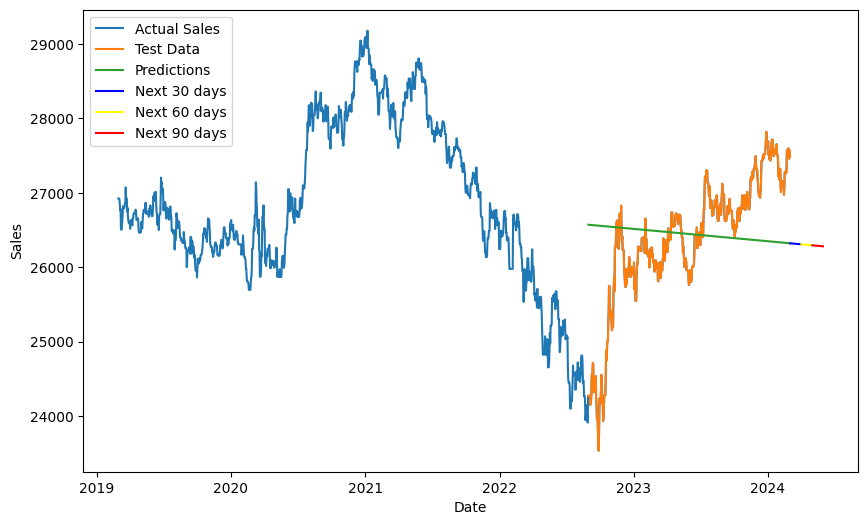
\includegraphics[width=\linewidth]{linear73_EUR.png}
    \caption{Linear model's result with 7:3 splitting proportion}
    \label{fig8}
  \end{minipage}
\end{figure}
\begin{figure}[H]
  \centering
  \begin{minipage}{0.8\linewidth}
    \centering
    \includegraphics[width=\linewidth]{bibliography/Figure/Stacking model/EUR_82_stacking.png}
    \caption{Stacking model's result with 8:2 splitting proportion}
    \label{fig9}
  \end{minipage}
\end{figure}
\begin{figure}[H]
  \centering
  \begin{minipage}{0.8\linewidth}
    \centering
    \includegraphics[width=\linewidth]{bibliography/GRU_VCB73.png}
    \caption{GRU model's result with 7:3 splitting proportion}
    \label{fig10}
  \end{minipage}
\end{figure}
\begin{figure}[H]
  \centering
  \begin{minipage}{0.8\linewidth}
    \centering
    \includegraphics[width=\linewidth]{ARIMA_EUR.png}
    \caption{ARIMA model's result with 9:1 splitting proportion}
    \label{fig11}
  \end{minipage}
\end{figure}
\begin{figure}[H]
  \centering
  \begin{minipage}{0.8\linewidth}
    \centering
    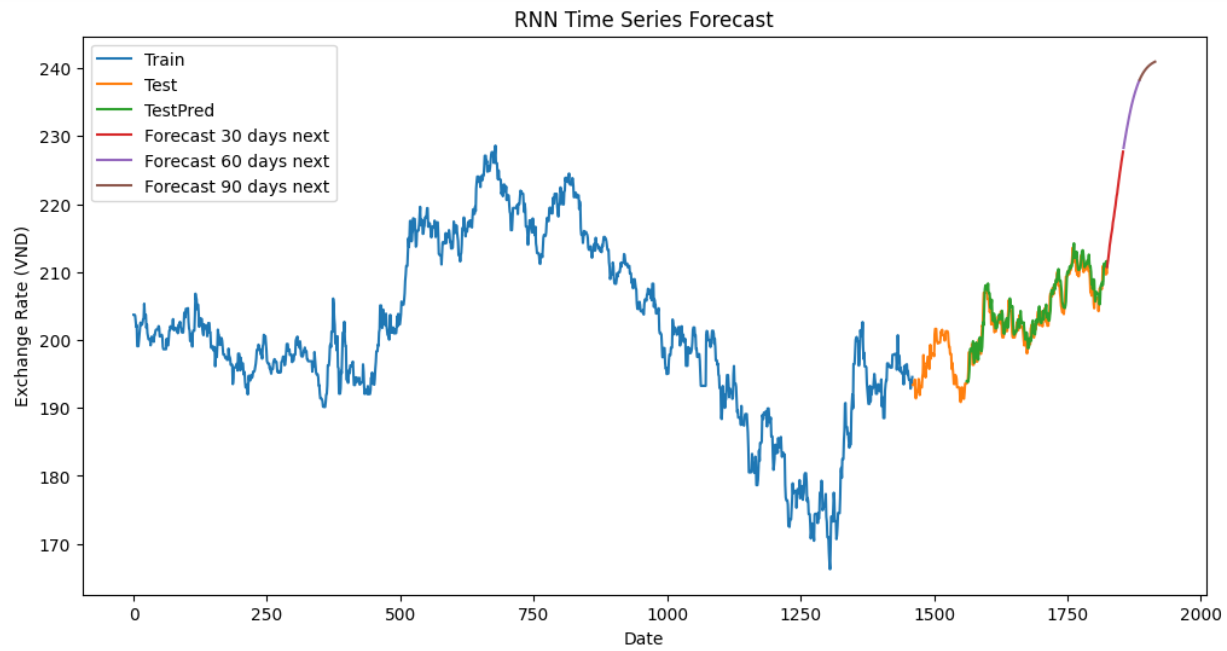
\includegraphics[width=\linewidth]{RNN_EUR.png}
    \caption{RNN model's result with 9:1 splitting proportion}
    \label{fig12}
  \end{minipage}
\end{figure}
\begin{figure}[H]
  \centering
  \begin{minipage}{0.8\linewidth}
    \centering
    \includegraphics[width=\linewidth]{bibliography/DLM_VCB82.png}
    \caption{DLM model's result with 8:2 splitting proportion}
    \label{fig13}
  \end{minipage}
\end{figure}
\begin{figure}[H]
  \centering
  \begin{minipage}{0.8\linewidth}
    \centering
    \includegraphics[width=\linewidth]{bibliography/ETS_VCB91.png}
    \caption{SES model's result with 9:1 splitting proportion}
    \label{fig14}
  \end{minipage}
\end{figure}
\begin{figure}[H]
  \centering
  \begin{minipage}{0.8\linewidth}
    \centering
    \includegraphics[width=\linewidth]{bibliography/baggingGRU_vcb.png}
    \caption{Bagging-GRU model's result with 8:2 splitting proportion}
    \label{bagginggru}
  \end{minipage}
\end{figure}
\subsection{GBP-VND dataset} 
\begin{table}[H]
    \centering
    \begin{tabular}{|c|c|c|c|c|}
         \hline
         \centering Model & Train:Test:Validate & RMSE & MAPE (\%) & MAE\\
         \hline
         \multirow{2}{*}{LN} &\ 7:3  &\ 1625.412 &\ 4.390 &\ 1277.908  \\ &\textbf{8:2} &\textbf{950.107} &\textbf{2.598} &\textbf{804.7} \\&\ 9:1 &\ 1165.593 &\ 3.26 &\ 1026.264 \\
         \hline
         \multirow{2}{*}{ARIMA} &\ 7:3 &\ 2391.128&\ 7.061 &\ 2160.296 \\ &\ 8:2 &\ 1865.457 &\ 5.445 &\ 1689.997 \\&\ \textbf{9:1} &\ \textbf{546.792} &\ \textbf{1.575} &\ \textbf{490.115} \\
         \hline
         \multirow{2}{*}{ETS} &\textbf{7:3} &\textbf{?}&\textbf{?}&\textbf{?} \\ &\ 8:2 &\ ?&\ ? &\ ? \\&\ 9:1 &\ ? &\ ? &\ ? \\
         \hline
         \multirow{2}{*}{RNN} & 7:3 & 1.465 & 0.544 & 1.107  \\ & 8:2 & 1.462 & 0.528 & 1.106 \\&\textbf{ 9:1} & \textbf{1.354} &\textbf{ 0.476} &\textbf{ 1.023} \\
         \hline
         \multirow{2}{*}{GRU} &\textbf{7:3} &\textbf{?}&\textbf{?}&\textbf{?} \\ &\ 8:2 &\ ?&\ ? &\ ? \\&\ 9:1 &\ ? &\ ? &\ ? \\
         \hline
         \multirow{2}{*}{Stacking Model} &\ 7:3 &\ 1620.452&\ 1429.037&\ 4.713 \\ &\ 8:2 &\ 817.089&\ 680.45 &\ 2.234 \\&\textbf{9:1} &\textbf{733.845} &\textbf{594.598} &\textbf{1.893} \\
         \hline
         \multirow{2}{*}{LSTM} &\textbf{7:3} &\textbf{?}&\textbf{?}&\textbf{?} \\ &\ 8:2 &\ ?&\ ? &\ ? \\&\ 9:1 &\ ? &\ ? &\ ? \\
         \hline
         \multirow{2}{*}{BatchTST} &\textbf{7:3} &\textbf{?}&\textbf{?}&\textbf{?} \\ &\ 8:2 &\ ?&\ ? &\ ? \\&\ 9:1 &\ ? &\ ? &\ ? \\
         \hline
    \end{tabular}
    \caption{GBP-VND Dataset's Evaluation}
    \label{mbbresult}
\end{table}

\begin{figure}[H]
  \centering
  \begin{minipage}{0.8\linewidth}
    \centering
    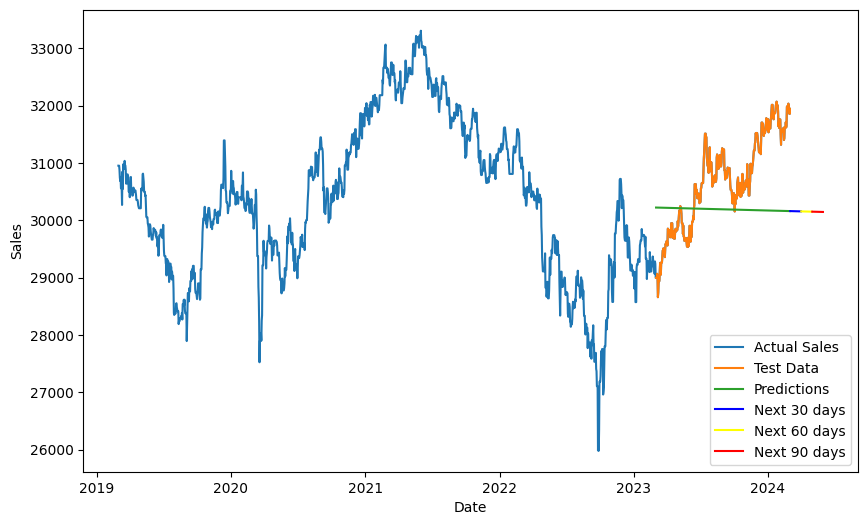
\includegraphics[width=\linewidth]{linear82_GBP.png}
    \caption{Linear model's result with 8:2 splitting proportion}
    \label{fig15}
  \end{minipage}
\end{figure}
\begin{figure}[H]
  \centering
  \begin{minipage}{0.8\linewidth}
    \centering
    \includegraphics[width=\linewidth]{bibliography/Figure/Stacking model/GBP_91_stacking.png}
    \caption{Stacking model's result with 9:1 splitting proportion}
    \label{fig16}
  \end{minipage}
\end{figure}
\begin{figure}[H]
  \centering
  \begin{minipage}{0.8\linewidth}
    \centering
    \includegraphics[width=\linewidth]{bibliography/GRU_MBB91.png}
    \caption{GRU model's result with 9:1 splitting proportion}
    \label{fig17}
  \end{minipage}
\end{figure}
\begin{figure}[H]
  \centering
  \begin{minipage}{0.8\linewidth}
    \centering
    \includegraphics[width=\linewidth]{ARIMA_GBP.png}
    \caption{ARIMA model's result with 9:1 splitting proportion}
    \label{fig18}
  \end{minipage}
\end{figure}
\begin{figure}[H]
  \centering
  \begin{minipage}{0.8\linewidth}
    \centering
    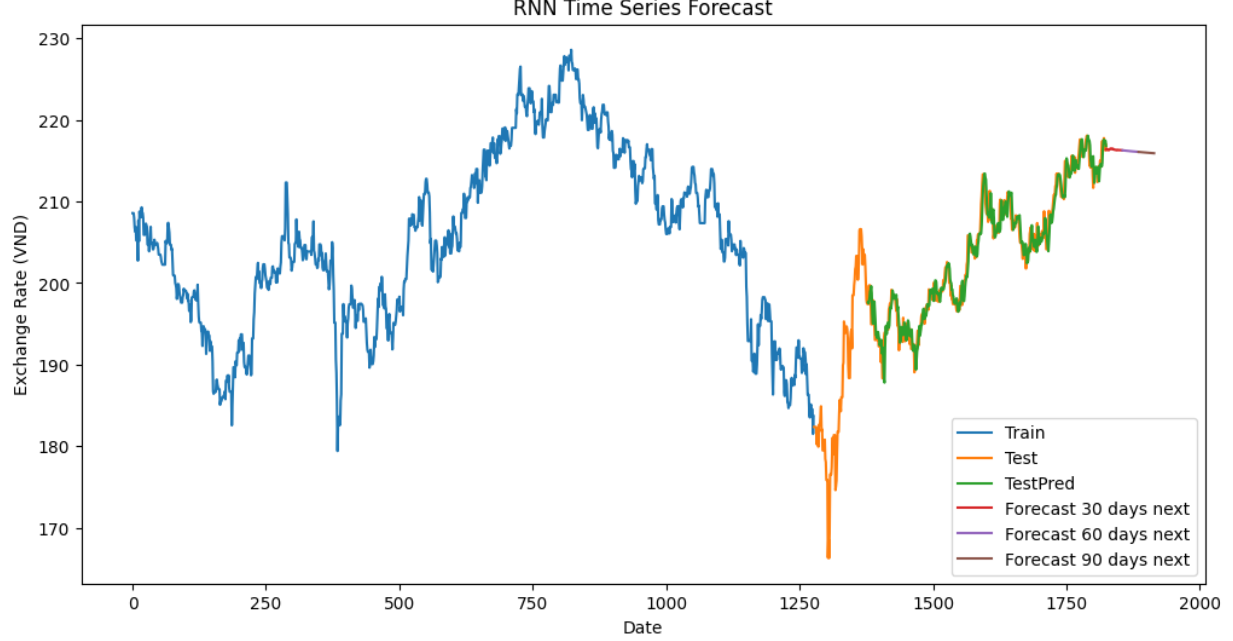
\includegraphics[width=\linewidth]{RNN_GBP.png}
    \caption{RNN model's result with 9:1 splitting proportion}
    \label{fig19}
  \end{minipage}
\end{figure}
\begin{figure}[H]
  \centering
  \begin{minipage}{0.8\linewidth}
    \centering
    \includegraphics[width=\linewidth]{bibliography/DLM_MBB91.png}
    \caption{DLM model's result with 9:1 splitting proportion}
    \label{fig20}
  \end{minipage}
\end{figure}
\begin{figure}[H]
  \centering
  \begin{minipage}{0.8\linewidth}
    \centering
    \includegraphics[width=\linewidth]{bibliography/ETS_MBB91.png}
    \caption{SES model's result with 9:1 splitting proportion}
    \label{fig21}
  \end{minipage}
\end{figure}
\begin{figure}[H]
  \centering
  \begin{minipage}{0.8\linewidth}
    \centering
    \includegraphics[width=\linewidth]{bibliography/baggingGRU_MBB.png}
    \caption{Bagging-GRU model's result with 9:1 splitting proportion}
    \label{mbbbggg}
  \end{minipage}
\end{figure}
\subsection{JPY-VND dataset} 
\begin{table}[H]
    \centering
    \begin{tabular}{|c|c|c|c|c|}
         \hline
         \centering Model & Train:Test:Validate & RMSE & MAPE (\%) & MAE\\
         \hline
         \multirow{2}{*}{LN} &\ 7:3 &\ 15.557 &\ 8.46 &\ 14.665 \\ &\ 8:2 &\ 7.39 &\ 3.791 &\ 6.491 \\&\textbf{9:1} &\textbf{4.749} &\textbf{2.399} &\textbf{4.078} \\
         \hline
         \multirow{2}{*}{ARIMA} &\ 7:3 &\ 8.645 &\ 4.284 &\ 7.6 \\ &\ 8:2 &\ 8.343 &\ 4.368 &\ 7.469  \\ &\textbf{9:1} &\textbf{2.749} &\textbf{1.264} &\textbf{2.173} \\
         \hline
         \multirow{2}{*}{ETS} &\textbf{7:3} &\textbf{?}&\textbf{?}&\textbf{?} \\ &\ 8:2 &\ ?&\ ? &\ ? \\&\ 9:1 &\ ? &\ ? &\ ? \\
         \hline
         \multirow{2}{*}{RNN} &  7:3  & 1.592 & 0.663 &\ 1.1698 \\ & 8:2  & 1.635  & 0.755  & 1.29 \\&\textbf{9:1} &\textbf{1.516} &\textbf{0.672} &\textbf{1.161} \\
         \hline
         \multirow{2}{*}{GRU} &\textbf{7:3} &\textbf{?}&\textbf{?}&\textbf{?} \\ &\ 8:2 &\ ?&\ ? &\ ? \\&\ 9:1 &\ ? &\ ? &\ ? \\
         \hline
         \multirow{2}{*}{Stacking Model} &\ 7:3 &\ 1928.667 &\ 17.7 &\ 10.181 \\ &\textbf{8:2} &\textbf{6.196} &\textbf{4.921} &\textbf{2.858} \\&\ 9:1 &\ 11.974 &\ 10.704 &\ 6.28 \\
         \hline
         \multirow{2}{*}{LSTM} &\textbf{7:3} &\textbf{?}&\textbf{?}&\textbf{?} \\ &\ 8:2 &\ ?&\ ? &\ ? \\&\ 9:1 &\ ? &\ ? &\ ? \\
         \hline
         \multirow{2}{*}{BatchTST} &\textbf{7:3} &\textbf{?}&\textbf{?}&\textbf{?} \\ &\ 8:2 &\ ?&\ ? &\ ? \\&\ 9:1 &\ ? &\ ? &\ ? \\
         \hline
    \end{tabular}
    \caption{JPY-VND Dataset's Evaluation}
    \label{mbbresult}
\end{table}

\begin{figure}[H]
  \centering
  \begin{minipage}{0.8\linewidth}
    \centering
    \includegraphics[width=\linewidth]{bibliography/Figure/Stacking model/linear_91_JPY.png}
    \caption{Linear model's result with 9:1 splitting proportion}
    \label{fig22}
  \end{minipage}
\end{figure}
\begin{figure}[H]
  \centering
  \begin{minipage}{0.8\linewidth}
    \centering
    \includegraphics[width=\linewidth]{bibliography/Figure/Stacking model/JPY_82_stacking.png}
    \caption{Stacking model's result with 8:2 splitting proportion}
    \label{fig23}
  \end{minipage}
\end{figure}
\begin{figure}[H]
  \centering
  \begin{minipage}{0.8\linewidth}
    \centering
    \includegraphics[width=\linewidth]{bibliography/GRU_BIDV91.png}
    \caption{GRU model's result with 9:1 splitting proportion}
    \label{fig24}
  \end{minipage}
\end{figure}
\begin{figure}[H]
  \centering
  \begin{minipage}{0.8\linewidth}
    \centering
    \includegraphics[width=\linewidth]{ARIMA_JPY.png}
    \caption{ARIMA model's result with 9:1 splitting proportion}
    \label{fig25}
  \end{minipage}
\end{figure}
\begin{figure}[H]
  \centering
  \begin{minipage}{0.8\linewidth}
    \centering
    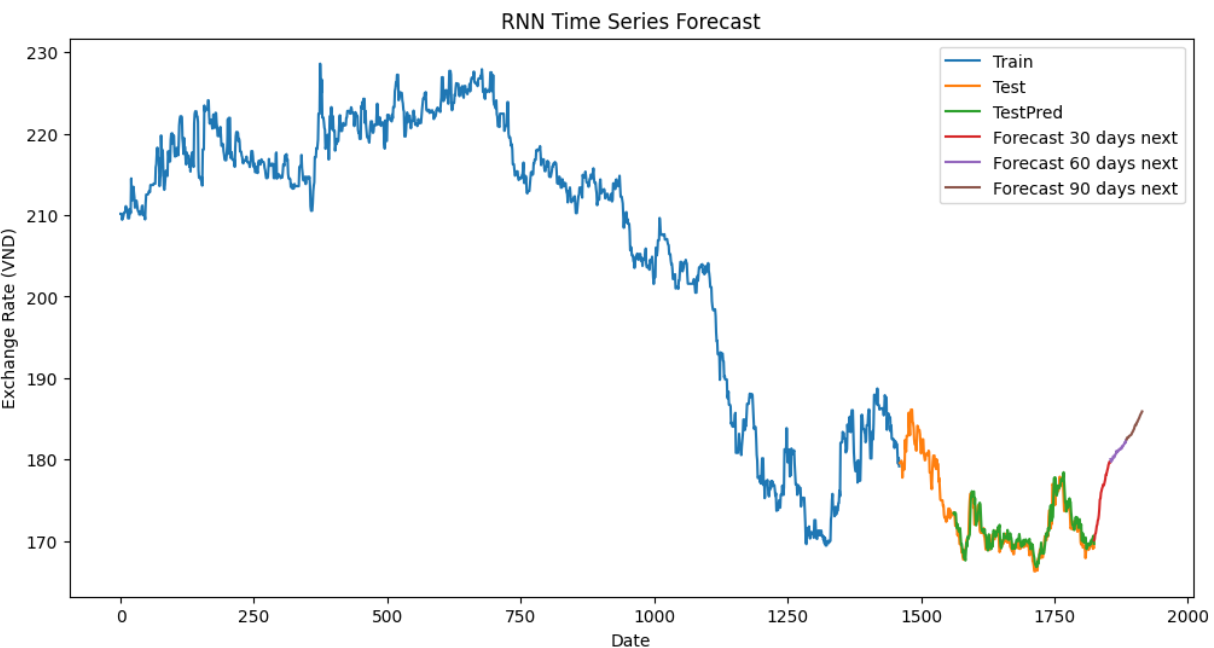
\includegraphics[width=\linewidth]{RNN_JPY.png}
    \caption{RNN model's result with 9:1 splitting proportion}
    \label{fig26}
  \end{minipage}
\end{figure}
\begin{figure}[H]
  \centering
  \begin{minipage}{0.8\linewidth}
    \centering
        \includegraphics[width=\linewidth]{bibliography/BIDV_DLM91.png}
    \caption{DLM model's result with 9:1 splitting proportion}
    \label{fig27}
  \end{minipage}
\end{figure}
\begin{figure}[H]
  \centering
  \begin{minipage}{0.8\linewidth}
    \centering
        \includegraphics[width=\linewidth]{bibliography/ETS_BIDV91.png}
    \caption{SES model's result with 9:1 splitting proportion}
    \label{fig28}
  \end{minipage}
\end{figure}
\begin{figure}[H]
  \centering
  \begin{minipage}{0.8\linewidth}
    \centering
        \includegraphics[width=\linewidth]{bibliography/baggingGRU_BIDV.png}
    \caption{Bagging-GRU model's result with 7:3 splitting proportion}
    \label{fig28}
  \end{minipage}
\end{figure}
\section{Conclusion}
Kết luận mẫu ---- Xóa dòng này
\subsection{Summary}
In the achievement of forecasting stock prices, the exploration of diverse methodologies, ranging from traditional statistical models to advanced machine learning algorithms, has been aimed. Among the performed models, Linear Regression (LR), Auto Regressive Integrated Moving Average (ARIMA), Support Vector Regression (SVR), Seasonal Auto Regression Integrated Moving Average (SARIMA), Dynamic Linear Model (DLM), Bagging – GRU, and Simple Exponential Smoothing (SES), it becomes evident that Support Vector Regression (SVR), Gated Recurrent Unit (GRU), and Bagging GRU emerge as the most promising and effective models for predicting stock prices.\\
The intricacies of stock price forecasting, rooted in the complexity and unpredictability of financial markets, demand models that can capture nuanced patterns and relationships within the data. Support Vector Regression (SVR) showcases its efficacy in handling intricate relationships, providing robust predictions. Gated Recurrent Unit (GRU) models, with their ability to capture sequential dependencies, exhibit notable performance in forecasting stock prices. The introduction of ensemble learning through Bagging GRU further refines the predictive capabilities, offering a collective insight that surpasses individual models.\\
As evidenced by the evaluation metrics, including RMSE, MAPE, and MSLE, the SVR, GRU, and Bagging GRU models consistently demonstrate superior performance across various aspects of forecasting accuracy. Their adaptability to handle the inherent uncertainties of stock markets positions them as formidable tools for investors and analysts seeking reliable predictions.
\subsection{Future Considerations}
In our future research, it is crucial to prioritize further optimization of the previously mentioned models. This optimization effort should specifically focus on:\\
\indent\textbullet\ Enhancing the accuracy of the model. While the above algorithms have demonstrated promising results in predicting stock prices, there is a need to further improve the model's accuracy to ensure more precise forecasting outcomes.\\
\indent\textbullet\ Exploring alternative machine learning algorithms or ensemble techniques. Ensemble techniques, such as combining multiple models or using various ensemble learning methods, can also improve the robustness and accuracy of the forecasts.\\
\indent\textbullet\ Researching new forecasting models. The field of forecasting continuously evolves, with new algorithms and models being researched and developed. It is crucial to stay updated with these approaches and explore new forecasting models that offer improved accuracy and performance. \\
By continuously exploring and incorporating new features, data sources, and modeling techniques, we can strive for ongoing optimization of the forecasting models and enhance their ability to predict stock prices with greater precision and reliability.
\section*{Acknowledgment}
\addcontentsline{toc}{section}{Acknowledgment}
First and foremost, we would like to express our sincere gratitude to \textbf{Assoc. Prof. Dr. Nguyen Dinh Thuan} and \textbf{Mr. Nguyen Minh Nhut} for their exceptional guidance, expertise, and invaluable feedback throughout the research process. Their mentorship and unwavering support have been instrumental in shaping the direction and quality of this study. Their profound knowledge, critical insights, and attention to detail have significantly contributed to the success of this research.
\\This research would not have been possible without the support and contributions of our mentors. We would like to extend our heartfelt thanks to everyone involved for their invaluable assistance, encouragement, and belief in our research. Thank you all for your invaluable assistance and encouragement.

%% UNCOMMENT these lines below (and remove the 2 commands above) if you want to embed the bibliography.
\begin{thebibliography}{00}
%%[1]-[5]: related work (PA)
\bibitem{b1} Liu, Pengfei, Ze Wang, Daoqun Liu, Jingyang Wang, and Tiezhu Wang. “A CNN-STLSTM-AM Model for Forecasting USD/RMB Exchange Rate.” Journal of Engineering Research 11, no. 2 (June 1, 2023): 100079. https://doi.org/10.1016/j.jer.2023.100079
\bibitem{b2} “Foreign Exchange Currency Rate Prediction Using a GRU-LSTM Hybrid Network - ScienceDirect.” Accessed April 14, 2024. https://www.sciencedirect.com/science/article/pii/S2666222120300083#sec0022.
\bibitem{b3} Liu, Siyuan, Qiqian Huang, Mingchen Li, and Yunjie Wei. “A New LASSO-BiLSTM-Based Ensemble Learning Approach for Exchange Rate Forecasting.” Engineering Applications of Artificial Intelligence 127 (January 1, 2024): 107305. https://doi.org/10.1016/j.engappai.2023.107305.
\bibitem{b4} Zhu, Qimian. “Forecasting the US Dollar/Euro Exchange Rate Based on ARIMA Model.” Advances in Economics, Management and Political Sciences 15 (September 13, 2023): 369–78. https://doi.org/10.54254/2754-1169/15/20230951.
\bibitem{b5} Kamruzzaman, Joarder, and Ruhul Sarker. “ANN-Based Forecasting of Foreign Currency Exchange Rates” 3 (January 1, 2004).
\bibitem{b6} “Staying positive: challenges and solutions in using pure multiplicative ETS models | IMA Journal of Management Mathematics | Oxford Academic.” Accessed: May 05, 2024. [Online]. Available: https://academic.oup.com/imaman/advance-article/doi/10.1093/imaman/dpad028/7475884
\bibitem{b7} “Exponential Smoothing- Definition, Formula, Methods and Examples,” BYJUS. Accessed: May 05, 2024. [Online]. Available: https://byjus.com/maths/exponential-smoothing/
\bibitem{b8}“STAT481581 Introduction to Time Series Analysis.pdf.” Accessed: May 15, 2024. [Online]. Available: https://math.unm.edu/~lil/Stat581/8-ets.pdf
\bibitem{b9}  M. Rahman, Md. S. Hossain, T.-S. Junaid, M. Forhad, and M. Hossen, “Predicting Prices of Stock Market using Gated Recurrent Units (GRUs) Neural Networks,” vol. 19, pp. 213–222, Jan. 2019.
\bibitem{b10} M. Yurtsever, “Gold Price Forecasting Using LSTM, Bi-LSTM and GRU,” European Journal of Science and Technology, Dec. 2021, doi: 10.31590/ejosat.959405
\bibitem{b10} Buja, A., and Stuetzle, W. ''Observations on bagging''. University of Pennsylvania and University of Washington, Seattle. 2002.
\bibitem{b11} B. M. Henrique, V. A. Sobrero, and H. Kimura, ``Comparison Of Fuzzy Time Series And ARIMA'', August 2019. Available:https://www.ijstr.org/final-print/aug2019/Comparison-Of-Fuzzy-Time-Series-And-Arima-Model.pdf. [Accessed 19 June 2023]. 4
\bibitem{b12} Jason Brownlee, ``How to Create an ARIMA Model for Time Series Forecasting in Python'', November 18, 2023. Available:https://www.ijstr.org/final-print/aug2019/Comparison-Of-Fuzzy-Time-Series-And-Arima-Model.pdf. 
\bibitem{b13} Jason Brownlee, ``A Gentle Introduction to SARIMA for Time Series Forecasting in Python'', August 21, 2019. 
\bibitem{b14} Alexandra M. Schmidt and Hedibert F. Lopes, ''Dynamic models'', 2019. 
\bibitem{b15} Timothy O. Hodson, ''Root-mean-square error (RMSE) or mean absolute error (MAE): when to use them or not'', 2022, https://doi.org/10.5194/gmd-15-5481-2022.
\bibitem{b16} Priya Pedamkar,''Support Vector Regression'', March 24, 2023. Retrieved from \(https://www.educba.com/support-vector-regression/?fbclid=IwAR0ibzdmqpaaDKq2-Q4JRcjxQcVt-C7TrHNEc90q_tCSrn8rds9x2AG8Y78\)
\bibitem{b17} Seok-Ho Han, Husna Mutahira, Hoon-Seok Jang, "Prediction of Sensor Data in a Greenhouse for Cultivation of Paprika Plants Using a Stacking Ensemble for Smart Farms", Applied Sciences, vol.13, no.18, pp.10464, 2023.

\end{thebibliography}
%%%%%%%%%%%%%%%


\EOD

\end{document}
